\documentclass[11pt]{article}
\newcommand{\ddd}{February 19, 2024}
\input{24aac-macro}

\begin{document}
\begin{center}
  \textbf{Topic 1: Series}
\end{center}

A (real) \textsf{series} is a formal sum $\sum_k a_k$ where the terms $a_k$ are real numbers.
The \textsf{$n^{\text{th}}$-partial sum} of the series is
\[
  S_n = a_0 + a_1 + \cdots + a_n.
\]
The series \textsf{converges} to a real number $S$ if $S_n \to S$ as $n \to \infty$, and we write
\[
  S = \sum_{k=0}^\infty a_k.
\]
A series that does not converge \textsf{diverges}.
The basic question to ask about a series is, does it converge or diverge?

\medskip
\noindent\textbf{Example.} Let $\lambda$ be a constant with $|\lambda| < 1$.
The \textit{geometric series} 
\[
  \sum_{k=0}^\infty \lambda^k = 1 + \lambda + \cdots + \lambda^n + \cdots
\]
converges to $\dfrac{1}{1-\lambda}$.
For its partial sums are
\[
  \Lambda_n = 1 + \lambda + \cdots + \lambda^n = \frac{1 - \lambda^{n+1}}{1 - \lambda} \to \frac{1}{1 - \lambda} \qquad \text{as $n \to \infty$}.
\]
On the other hand, if $|\lambda|\geqslant1$ then the series $\sum_k \lambda^k$ diverges.

\medskip
Since the convergence of a series is defined via that of its partial sum sequences, the Cauchy criterion for sequences can directly be applied here.
We state the result without providing its proof.

\begin{prop}[Cauchy criterion for series]
  A series $\sum_k a_k$ converges if and only if for any $\varepsilon > 0$ there is an integer $N \in \mathbb{N}$ such that whenever $m \geqslant n \geqslant N$,
  \[
    \left| \sum_{k=n}^m a_k \right| = |a_n + \cdots + a_m| < \varepsilon.
  \]
\end{prop}

One immediate consequence for the Cauchy criterion for series is that no finite number of terms affects convergence of a series.
Rather, it is the \textit{tail} of the series, the terms $a_k$ with $k$ large, that determines convergence or divergence.
Likewise, whether the series leads off with a term of index $k = 0$ or $k = 1$, etc., does not matter.
Another useful and simple check is the following result.

\begin{cor}[Zero test for series]
  \label{cor:zero-test}
  Let $\sum_k a_k$ be a convergent series.
  Then $a_k \to 0$ as $k \to \infty$.
\end{cor}

\begin{proof}
  Take $n = m$ in the Cauchy criterion for series:
  \[
    \left| \sum_{k=m}^m a_k \right| = |a_m| < \varepsilon
  \]
  whenever $m \geqslant N$.
\end{proof}

Note that Corollary~\ref{cor:zero-test} only states a \textit{necessary} condition for convergence of series; the zero test is not sufficient to guarantee the convergence of series.
See the $p$-series below.

The linear properties for convergent series are clear.
We state them as a theorem below without their proofs.
\begin{thm}
  Let $\sum_k a_k$ and $\sum_k b_k$ be convergent series, and $\lambda \in \mathbb{R}$ be a constant.  Then the following identities hold.
  \begin{enumerate}[(i)]
    \item $\displaystyle \sum_k (a_k + b_k) = \sum_k a_k + \sum_k b_k$.

    \item $\displaystyle \sum_k \lambda a_k = \lambda \sum_k a_k$.
  \end{enumerate}
\end{thm}

There are many tests to tell whether a series converges or not.
On the contrary, the limit to which the series converge can be very hard to identify.
Almost all convergence tests boil down to the following result.

\begin{thm}[Comparison test for series]
  If a series $\sum_k b_k$ \textsf{dominates} a series $\sum_k a_k$ in the sense that for all sufficiently large $k$ we have $|a_k| \leqslant b_k$ then the convergence of $\sum_k b_k$ implies convergence of $\sum_k a_k$.
\end{thm}

\begin{proof}
  Given $\varepsilon > 0$, convergence of $\sum_k b_k$ implies that there is a large $N$ such that for all $m \geqslant n \geqslant N$ we have $\sum_{k=n}^m b_k < \varepsilon$.  (Note that the assumption $|a_k| \leqslant b_k$ implicitly verifies that $b_k \geqslant 0$.)
  Thus,
  \[
    \left| \sum_{k=n}^m a_k \right| \leqslant \sum_{k=n}^m |a_k| \leqslant \sum_{k=n}^m b_k < \varepsilon.
  \]
  And convergence of $\sum_k a_k$ follows from the Cauchy criterion for series.
\end{proof}

\noindent\textbf{Example.} The series $\sum_k \sin(k) / 2^k$ converges since it is dominated by the convergent geometric series $\sum_k 1/2^k$.

\medskip
A series $\sum_k a_k$ converges \textsf{absolutely} if $\sum_k |a_k|$ converges.
The comparison test shows that absolute convergence implies convergence.
A convergent series that does not converge absolutely is said to converge \textsf{conditionally}.
Examples will be given below.

Series and integrals are both infinite sums.
You can imagine a series as an improper integral in which the integration variable is an integer, that is,
\[
  \sum_{k=0}^\infty a_k = \int_{\mathbb{N}} a_k \, \dd k.
\]
More precisely, given a series $\sum_k a_k$, define a function $f: [0,\infty) \to \mathbb{R}$ by setting
\[
  f(x) = a_k, \qquad x \in (k-1, k],
\]
for any $k \in \mathbb{N}$.
Then
\[
  \sum_{k=1}^\infty a_k = \int_0^\infty f(x) \, \dd x.
\]
The series converges if and only if the improper integral does, as the following theorem states.
\begin{thm}[Integral test]
  Suppose that $\int_0^\infty f$ is a given improper integral and $\sum_k a_k$ is a given series.
  \begin{enumerate}[(i)]
    \item If $|a_k| \leqslant f(x)$ for all sufficiently large $k$ and all $x \in (k-1,k]$ then convergence of the improper integral implies convergence of the series.
  \item If $|f(x)| \leqslant a_k$ for all sufficiently large $k$ and all $x \in [k, k+1)$ then divergence of the improper integral implies divergence of the series.
  \end{enumerate}
\end{thm}

\begin{proof}
  \begin{enumerate}[(i)]
    \item For some large $N_0$ and all $N \geqslant N_0$ we have
      \[
	\sum_{k=N_0+1}^N |a_k| \leqslant \int_{N_0}^N f \leqslant \int_0^\infty f,
      \]
      which is a finite real number.
      An increasing, bounded sequence converges to a limit by the monotone convergence theorem, so the tail of the series $\sum_k |a_k|$ converges and the whole series $\sum_k |a_k|$ converges as well.
      Absolute convergence implies convergence.
  \end{enumerate}

  \medskip
  The proof of (ii) is similar and left to readers.
\end{proof}

\noindent\textbf{Example.} The \textsf{$p$-series} $\sum_k 1/k^p$ converges when $p > 1$ but diverges when $0 < p \leqslant 1$.

For this let us examine the improper integral $\int_1^\infty 1/x^p \, \dd x$.
A direct calculation gives, for $p > 0$,
\[
  \int_1^b \frac{1}{x^p} \, \dd x = 
  \begin{cases}
    \dfrac{b^{1-p}-1}{1-p}, & \text{if $p \ne 1$}; \\
    \ln b                , & \text{if $p = 1$}.
  \end{cases}
\]
These quantities converges (to $\frac{1}{p-1}$) when $p>1$, but blows up when $0 < p \leqslant 1$.  The results follow.

Note that the $p$-series for $0 < p \leqslant 1$ give counterexamples for sufficiency for the zero test: $1/k^p \to 0$ as $k \to \infty$, but $\sum_k 1/k^p$ diverges.

\begin{defn}
  Let $\sum_k a_k$ be a real series.
  The \textsf{exponential growth rate} of the series $\sum_k a_k$ is
  \[
    \alpha = \limsup_{n\to\infty} \sqrt[k]{|a_k|} \in [0,\infty].
  \]
\end{defn}

For example, $\sum_k \alpha^k$ has the exponential growth rate $|\alpha|$.

\begin{thm}[Root test]
  Let $\alpha$ be the exponential growth rate of a series $\sum_k a_k$.
  \begin{enumerate}[(i)]
    \item If $\alpha < 1$, then $\sum_k a_k$ converges.

    \item If $\alpha > 1$, then $\sum_k a_k$ diverges.

    \item If $\alpha = 1$, the root test is inconclusive: $\sum_k a_k$ could be convergent or divergent.
  \end{enumerate}
\end{thm}

\begin{proof}
  \begin{enumerate}[(i)]
    \item Suppose $\alpha < 1$.  Fix a number $\beta$ such that $\alpha < \beta < 1$.
      Then for sufficiently large $k$ we have $|a_k|^{1/k} < \beta$, i.e., $|a_k| < \beta^k$, which gives convergence of $\sum_k a_k$ by comparison to the convergent geometric series $\sum_k \beta^k$.

    \item Suppose $\alpha > 1$.  Again fix a number $\beta$ such that $1 < \beta < \alpha$.  Then there are infinitely many $k$ such that $|a_k|^{1/k} > \beta$, i.e., $|a_k| > \beta^k > 1$ infinitely often.
      Hence $\sum_k a_k$ must diverge because it fails the zero test.
    
    \item This statement is not vacuous: we have two series, one convergent but the other divergent, whose exponential growth rates are both $1$.
      The examples are the $p$-series: it converges when $p > 1$, but diverges when $0 < p \leqslant 1$.
  \end{enumerate}
\end{proof}

\begin{thm}[Ratio test]
  Let the ratio between successive terms of the series $\sum_k a_k$ be $r_k = | a_{k+1} / a_k |$, and set
  \[
    \limsup_{k\to\infty} r_k = \rho, \quad
    \liminf_{k\to\infty} r_k = \lambda.
  \]
  \begin{enumerate}[(i)]
    \item If $\rho < 1$, then $\sum_k a_k$ converges.

    \item If $\lambda > 1$, then $\sum_k a_k$ diverges.

    \item Otherwise, the ratio test is inconclusive.
  \end{enumerate}
\end{thm}

\begin{proof}
  \begin{enumerate}[(i)]
    \item Suppose $\rho < 1$.  Fix a number $\beta$ such that $\rho < \beta < 1$.  Then there is a positive integer $K$ such that $r_k < \beta$, i.e., $|a_{k+1}| < \beta |a_k|$, whenever $k \geqslant K$.
      By mathematical induction we conclude that
     \[
       |a_{K+n}| < |a_K| \beta^n
     \]
     for all $n \in \mathbb{N}$.  Hence $\sum_k a_k$ converges by comparison to the convergent geometric series $\sum_k |a_K| \beta^k$.

   \item Suppose $\lambda > 1$.  Again fix a number $\beta$ such that $1 < \beta < \lambda$.  Then there is a positive integer $K \in \mathbb{N}$ such that $r_k > \beta$, i.e., $|a_{k+1}| > \beta |a_k| > |a_k|$ whenever $k \geqslant K$.  Thus $\sum_k a_k$ must diverge for it fails the zero test.

   \item Again the $p$-series provide examples for the inconclusion for the ratio test.
  \end{enumerate}
\end{proof}

\noindent\textbf{Example.}
    Consider the series $\sum_k a_k$, where the terms $a_k$ are defined as
    \[
      a_k = \begin{cases}
        2^{-(k+1)/2}, & \text{if $k$ is odd}; \\
        3^{-k/2},     & \text{if $k$ is even}.
    \end{cases}
    \]
    That is, $\sum_k a_k = \frac12 + \frac13 + \frac1{2^2} + \frac1{3^2} + \frac1{2^3} + \frac1{3^3} + \cdots$.
    A direct computation shows
    \begin{align*}
      \liminf_{k\to\infty} \frac{a_{k+1}}{a_k} = 0, & & \limsup_{k\to\infty} \frac{a_{k+1}}{a_k} = \infty; \\
      \liminf_{k\to\infty} \sqrt[k]{a_k} = \frac{1}{\sqrt{3}}, & & \limsup_{k\to\infty} \sqrt[k]{a_k} = \frac{1}{\sqrt{2}}.
    \end{align*}
    That is, while the root test says that the series $\sum_k a_k$ converges, the ratio test is inconclusive.


\section*{Absolute convergence and conditional convergence}

\begin{defn}
  Let $\sum_k a_k$ be a real series.
  \begin{enumerate}[(i)]
    \item $\sum_k a_k$ is said to \textsf{converge absolutely} if $\sum_k |a_k|$ converges.

    \item $\sum_k a_k$ is said to \textsf{converge conditionally} if it converges but not converges absolutely.
  \end{enumerate}
\end{defn}

A bit of objection here.
When we say a series $\sum_k a_k$ converges absolutely, we do not know whether the series itself converges or not.
The usage of ``absolutely'' as an adverb seems inadequate.
The justification will be available once the following result is shown.

\begin{prop}
  If a series $\sum_k a_k$ converges absolutely, it converges.
  Furthermore, we have $| \sum_k a_k | \leqslant \sum_k |a_k|$.
\end{prop}

\begin{proof}
  This is clear from Cauchy criterion, since whenever $n \geqslant m$, we have
  \[
    \left| \sum_{k=m}^n a_k \right| \leqslant \sum_{k=m}^n |a_k|
  \]
  by the triangle inequality.
  
  For the comparison of their limits, we note that
  \[
    0 \leqslant |a_k| + a_k \leqslant 2 |a_k|.
  \]
  Hence by the comparison theorem
  \[
    \sum_k |a_k| + \sum_k a_k \leqslant 2 \sum_k |a_k|,
  \]
  and the result follows.
\end{proof}

In finite sums, the orders of terms do not affect the result because of the commutativity of addition.
Also parentheses can be used to group terms in an arbitrary way.
However, the situation may not be the same for infinite series.
To describe what happens, we introduce the following terminology.

\begin{defn}
  A series $\sum_{k=1}^\infty b_k$ is called a \textsf{rearrangement} of a series $\sum_{k=1}^\infty a_k$ if and only if there is a bijection $f: \mathbb{N} \to \mathbb{N}$ such that
  \[
    b_{f(k)} = a_k, \qquad k \in \mathbb{N}.
  \]
\end{defn}
In plain words, a rearrangement of a series is a re-ordering of the original series such that each term appears exactly once in the new series.
The following result demonstrates why absolutely convergent are so important.

\begin{thm}
  If $\sum_k a_k$ converges absolutely and $\sum_k b_k$ is any rearrangement of $\sum_k a_k$, then $\sum_k b_k$ converges and 
  \[
    \sum_{k=1}^\infty b_k = \sum_{k=1}^\infty a_k.
  \]
\end{thm}

\begin{proof}
  Let $\varepsilon > 0$ be given.
  \begin{align*}
    s_n &= \sum_{k=1}^n a_k \to s \qquad \text{as $k \to \infty$}; \\
    t_m &= \sum_{k=1}^m b_k.
  \end{align*}
  Since $\sum_k a_k$ converges absolutely, we can choose $N \in \mathbb{N}$ such that
  \[
    \sum_{k=N+1}^\infty |a_k| < \frac{\varepsilon}{2}.
  \]
  Thus
  \[
    |s_N - s| = \left| \sum_{k=N+1}^\infty a_k \right| \leqslant \sum_{k=N+1}^\infty |a_k| < \frac{\varepsilon}{2}.
  \]

  Let $f$ be a bijection from $\mathbb{N}$ to $\mathbb{N}$ such that $b_{f(k)} = a_k$ for $k \in \mathbb{N}$, and set
  \[
    M = \max \{ f(k) \colon k = 1, 2, \dots, N \}.
  \]
  Note that from the definition of $M$ we have
  \[
    \{ a_1, a_2, \dots, a_N \} \subseteq \{ b_1, b_2, \dots, b_M \}.
  \]
  Let $m \geqslant M$.  Then $t_m - s_N$ contains only $a_k$'s whose indices satisfy $k > N$.  Thus
  \[
    |t_m - s_N| \leqslant \sum_{k=N+1}^\infty |a_k| < \frac{\varepsilon}{2}.
  \]
  Hence,
  \[
    |t_m - s| \leqslant |t_m - s_N| + |s_N - s| \leqslant \frac{\varepsilon}{2} + \frac{\varepsilon}{2} = \varepsilon
  \]
  for $m \geqslant M$.
  Therefore $\sum_{k=1}^\infty b_k = s$ as well.
\end{proof}

In the following let us discuss the situation for \textit{conditionally} convergent series informally.
For each real series $\sum_k a_k$, let us define for each $k$,
\[
  a_k^+ = \frac{|a_k|+a_k}{2} = 
  \begin{cases}
    a_k, & \text{when $a_k \geqslant 0$}, \\
    0,   & \text{when $a_k < 0$};
  \end{cases}
  \quad
  \text{and}
  \quad
  a_k^- = \frac{|a_k|-a_k}{2} = 
  \begin{cases}
    0,      & \text{when $a_k \geqslant 0$}, \\
    -a_k,   & \text{when $a_k < 0$}.
  \end{cases}
\]
The series $\sum_k a_k^+$ (resp.\ $\sum_k a_k^-$) is called the series of \textit{positive} terms (resp.\ \textit{negative} terms) of $\sum_k a_k$.
It is clear that $\sum_k |a_k| = \sum_k (a_k^+ + a_k^-)$ and $\sum_k a_k = \sum_k (a_k^+ - a_k^-)$.
Because both $\sum_k a_k^+$ and $\sum_k a_k^-$ are non-negative series, $\sum_k a_k$ converges absolutely if and only if both $\sum_k a_k^+$ and $\sum_k a_k^-$ converges.
However, the following lemma is an important observation for conditionally convergent series.

\begin{lem}
  Let $\sum_k a_k$ be a conditionally convergent series.
  Then both $\sum_k a_k^+$ and $\sum_k a_k^-$ diverge (to infinity).
\end{lem}

\begin{proof}
  At least one of $\sum_k a_k^+$ and $\sum_k a_k^-$ must diverge.
  If exactly one of them diverges, then the original series $\sum_k a_k$ diverges as well.
  Therefore both of them must diverge.
\end{proof}

Now suppose that $\sum_k a_k$ converges conditionally.
Using this lemma and the fact that $a_k \to 0$ and $k \to 0$ (the zero test), one can show that following result whose proof is left to interested readers.

\begin{thm}
  Let $\sum_k a_k$ be a conditionally convergent series.
  \begin{enumerate}[(i)]
    \item (Riemann) Given any real number $s \in \mathbb{R}$, there is a rearrangement $\sum_k b_k$ of $\sum_k a_k$ whose sum converges to $s$.

    \item Let $-\infty \leqslant \alpha \leqslant \beta \leqslant \infty$.
      There is a rearrangement $\sum_k c_k$ of $\sum_k a_k$ satisfying $\liminf_{n \to \infty} t_n = \alpha$ and $\limsup_{n \to \infty} t_n = \beta$ where $\langle t_n \rangle$ is the partial sum sequence of $\sum_k c_k$.
  \end{enumerate}
\end{thm}

\medskip
\noindent\textbf{\large Alternating series}

So far we discuss tools to determine convergence or divergence for non-negative series.
In this section we derive two tests to use on series whose terms have mixed signs.
Both tests rely on the following algebraic observation.

\begin{thm}[Abel's formula]
  Let $\langle a_k \rangle$ and $\langle b_k \rangle$ be real sequences.
  For each pair of integers $n \geqslant m \geqslant 1$ define
  \[
    A_{m,n} = \sum_{k=m}^n a_k.
  \]
  Then
  \[
    \sum_{k=m}^n a_k b_k = A_{m,n} b_n + \sum_{k=m}^{n-1} A_{m,k} (b_k - b_{k+1})
  \]
  for all integers $n \geqslant m \geqslant 1$.
\end{thm}

\begin{proof}
  Since $A_{m,m} = a_m$ and $a_k = A_{m,k} - A_{m,k-1}$ for $k > m$, we have
  \begin{align*}
    \sum_{k=m}^n a_k b_k &= a_m b_m + \sum_{k=m+1}^n a_k b_k \\
    &= A_{m,m} b_m + \sum_{k=m+1}^n (A_{m,k} - A_{m,k-1}) b_k \\
    &= \sum_{k=m}^{n-1} A_{m,k} (b_k - b_{k+1}) + A_{m,n} b_n. 
  \end{align*}
\end{proof}

\noindent\textit{Remark.} The Abel's formula is sometimes called \textit{summation by parts}, which is a discrete version of integration by parts.  Note their similarity.

\medskip
Our first application of Abel's formula is the following test.
Note that it does not require that the $a_k$'s be non-negative.

\begin{thm}[Dirichlet's test]
  Let $a_k, b_k \in \mathbb{R}$ for $k \in \mathbb{N}$.
  If the sequence of partial sums $s_n = \sum_{k=1}^n a_k$ is bounded and $b_k \searrow 0$ as $k \to \infty$, then $\sum_{k=1}^\infty a_k b_k$ converges.
\end{thm}

\begin{proof}
  Choose $M > 0$ such that
  \[
    |s_n| = \left| \sum_{k=1}^n a_k \right| \leqslant \frac{M}{2}, \quad n \in \mathbb{N}.
  \]
  By the triangle inequality,
  \[
    |A_{m,n}| = \left| \sum_{k=m}^n a_k \right| = |s_n - s_{m-1}| \leqslant \frac{M}{2} + \frac{M}{2} = M.
  \]
  for $n \geqslant m > 1$.

  Let $\varepsilon > 0$ and choose $N \in \mathbb{N}$ so that $0 \leqslant b_k < \dfrac{\varepsilon}{M}$ for $k \geqslant N$.
  Since $\langle b_k \rangle$ is decreasing and non-negative, we find, by Abel's formula, the choice of $M$, and by telescoping that
  \begin{align*}
    \left| \sum_{k=m}^n a_k b_k \right| &\leqslant |A_{m,n}| b_n + \sum_{k=m}^{n-1} |A_{m,k}| (b_k - b_{k+1}) \\
    &\leqslant M b_n + \sum_{k=m}^{n-1} M (b_k - b_{k+1}) \\
    &= M b_m < M \cdot \frac{\varepsilon}{M} = \varepsilon,
  \end{align*}
  whenever $n \geqslant m \geqslant N$.
  Since $\varepsilon$ is arbitrary, we conclude that $\sum_k a_k b_k$ converges by the Cauchy criterion.
\end{proof}

The following test is a direct application for the Dirichlet's test and is more widely known.

\begin{cor}[Alternating series test]
  If $b_k \searrow 0$ as $k \to 0$, then
  \[
    \sum_{k=1}^\infty (-1)^k b_k
  \]
  converges.
\end{cor}

This reason for this test being called the alternating series test is evident: the signs of the terms in this series are alternating between positive and negative.

\begin{proof}
  Simply take $\sum_{k=1}^\infty a_k = (-1) + 1 + (-1) + 1 + \cdots$.
  Note that the partial sums of $\sum_k a_k$ are either $-1$ or $0$, hence its partial sum sequence is bounded.
  Hence the Dirichlet's test applies.
\end{proof}

\noindent\textbf{\large Cauchy convolution product of series}

Two convergent series might be added term by term, and the resulting series converges to the sum of the two series.
The situation becomes more complicated when we consider multiplication of two series.
To begin with, we have to define the product.
This can be done in several ways; we shall consider the so-called Cauchy product.

\begin{defn}
  Given $\sum_k a_k$ and $\sum_k b_k$, we put
  \[
    c_n = \sum_{k=0}^n a_k b_{n-k}, \qquad n = 0, 1, 2, \dots.
  \]
  We call $\sum_k c_k$ the \textsf{(Cauchy) product} (or the \textsf{convolution product}) of the two given series.
\end{defn}

This definition may be motivated as follows.
We take two series $\sum_k a_k$ and $\sum_k b_k$, and form all possible products of the form $a_j b_k$. Below is an arrangement of these terms into a table:

\begin{center}
  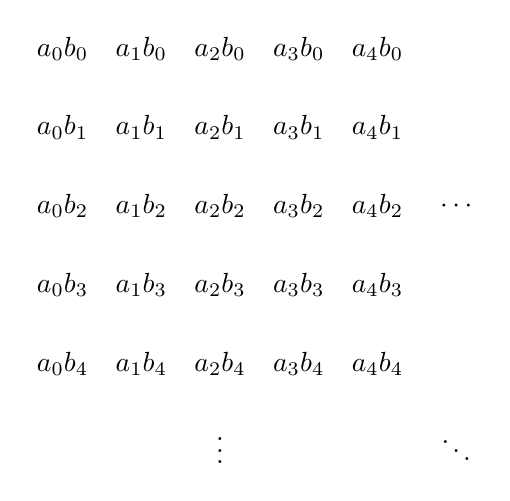
\begin{tikzpicture}
    \foreach \x in {0,1,2,3,4}
    \foreach \y in {0,1,2,3,4}
    \node at (\x, -\y) {$a_{\x} b_{\y}$};
    \node at (2,-5) {$\vdots$};
    \node at (5,-2) {$\cdots$};
    \node at (5,-5) {$\ddots$};
  \end{tikzpicture}
\end{center}
That is the expansion by the distributive law when we multiply these two series:
\[
  (a_0 + a_1 + a_2 + \cdots)(b_0 + b_1 + b_2 + \cdots) \rightarrow
  a_0 b_0 + a_0 b_1 + \cdots + a_1 b_0 + a_1 b_1 + \cdots.
\]
Of course we have not defined how to add such a series if one term appears after infinitely many terms, and this is why we use an arrow instead of an equal sign.
One way to add such a series is to collect terms along each anti-diagonal.
That is why we define $c_n = \sum_k a_k b_{n-k}$.
Here is a result about the convergence of the Cauchy product of two convergent series.

\begin{thm}[Mertens]
  Suppose $\sum_{k=0}^\infty a_k = A$ and $\sum_{k=0}^\infty b_k = B$ be two convergent series, and define $c_n = \sum_{k=0}^n a_k b_{n-j}$ for $n = 0, 1, 2, \dots$.
  If $\sum_k a_k$ converges absolutely, then
  \[
    \sum_{k=0}^\infty c_k = AB.
  \]
\end{thm}

That is, the product of two convergent series converges, and to the right value, if at least one of the two series converges absolutely.

\begin{proof}
  Put
  \[
    A_n = \sum_{k=0}^n a_n, \quad
    B_n = \sum_{k=0}^n b_n, \quad
    C_n = \sum_{k=0}^n c_n, \quad
    \beta_n = B_n - B.
  \]
  Then
  \begin{align*}
    C_n &= a_0 b_0 + (a_0 b_1 + a_1 b_0) + \cdots + (a_0 b_n + \cdots + a_n b_0) \\
    &= a_0 B_n + a_1 B_{n-1} + \cdots + a_n B_0 \\
    &= a_0 (B + \beta_n) + a_1 (B + \beta_{n-1}) + \cdots + a_n (B + \beta_0) \\
    &= A_n B + a_0 \beta_n + a_1 \beta_{n-1} + \cdots + a_n \beta_0.
  \end{align*}
  Set
  \[
    \gamma_n = a_0 \beta_n + a_1 \beta_{n-1} + \cdots + a_n \beta_0.
  \]

  We wish to show that $C_n \to AB$ as $n \to \infty$.  Since $A_n B \to AB$, it suffices to show that
  \begin{equation}
    \label{eq:gammaa}
    \lim_{n\to\infty} \gamma_n = 0.
  \end{equation}
  To prove (\ref{eq:gammaa}), we put
  \[
    \alpha = \sum_{k=0}^\infty |a_k|.
  \]
  Let $\varepsilon > 0$ be given.  Since $\sum_{k=0}^\infty b_k = B$, we see that $\beta_n \to 0$.  Hence we may choose $N \in \mathbb{N}$ such that $|\beta_n| \leqslant \varepsilon$ for any $n \geqslant N$.  Thus
  \begin{align*}
    |\gamma_n| &\leqslant |\beta_0 a_n + \cdots + \beta_N a_{n-N}| + |\beta_{N+1} a_{n-N-1} + \cdots + \beta_n a_0| \\
    &\leqslant |\beta_0 a_n + \cdots + \beta_N a_{n-N}| + \varepsilon \alpha.
  \end{align*}
  Keeping $N$ fixed and letting $n \to \infty$, we get
  \[
    \limsup_{n\to\infty} |\gamma_n| \leqslant \varepsilon \alpha,
  \]
  since $a_k \to 0$ as $k \to \infty$.  Since $\varepsilon$ is arbitrary, we have shown (\ref{eq:gammaa}).
\end{proof}

There is another set of hypotheses that guarantees the limit of convergent Cauchy product of two series is the right value.
We state the theorem here, but its proof may be delayed until the coming semester.
Note that it does not require absolute convergence of any series.

\begin{thm}
  If the series $\sum_k a_k$, $\sum_k b_k$, $\sum_k c_k$ converge to $A, B$ and $C$, respectively, where $c_n = a_0 b_n + a_1 b_{n-1} + \cdots + a_n b_0$ for $n = 0,1,2,\dots$, then $C = AB$.
\end{thm}

\medskip
So far we have discussed several basic tools to determine whether a real series converges or diverges.
Of course there are more advanced tools out there.
Perhaps one should master to these basic tools before trying out harder ones.

\end{document}
